\documentclass[11pt]{article}
\usepackage[margin=1in]{geometry}
\usepackage{graphicx}
\usepackage{booktabs}
\title{SCOREMAP: Structure-aware grading of handwritten CS answer scripts}
\author{Team group27}
\date{}
\begin{document}
\maketitle
\begin{abstract}
SCOREMAP converts handwritten CS answers into typed evidence graphs and executes rubrics over them to assign grounded partial credit.
\end{abstract}
\section{Introduction}
Handwritten CS scripts mix prose, pseudocode, complexity notation, and diagrams. SCOREMAP handles this with typed evidence extraction and executable rubrics.
\section{Related Work}
We study Donut, LayoutLMv3, and Pix2Struct as the main prior-work anchors.
\section{Dataset}
The included pilot benchmark contains 18 question-level samples across 6 question archetypes and 3 writer styles with writer-wise splits.
\section{Method}
The pipeline performs typed region extraction, evidence graph construction, rubric execution, and constrained score aggregation.
\section{Experiments}
We compare a generic scorer, a no-graph ablation, and the full SCOREMAP model.
\section{Results}
See Table~\ref{tab:main} and Figure~\ref{fig:comparison}.
\begin{table}[h]
\centering
\begin{tabular}{lcccc}
\toprule
Model & MAE & Kappa & Item F1 & Evidence F1 \\
\midrule
Generic & 2.0 & 0.1356 & 0.75 & 0.5 \\
No-graph & 1.6667 & 0.2 & 0.7273 & 0.5 \\
SCOREMAP & 1.3333 & 0.3878 & 0.7647 & 0.5417 \\
\bottomrule
\end{tabular}
\caption{Pilot benchmark results.}
\label{tab:main}
\end{table}
\begin{figure}[h]
\centering
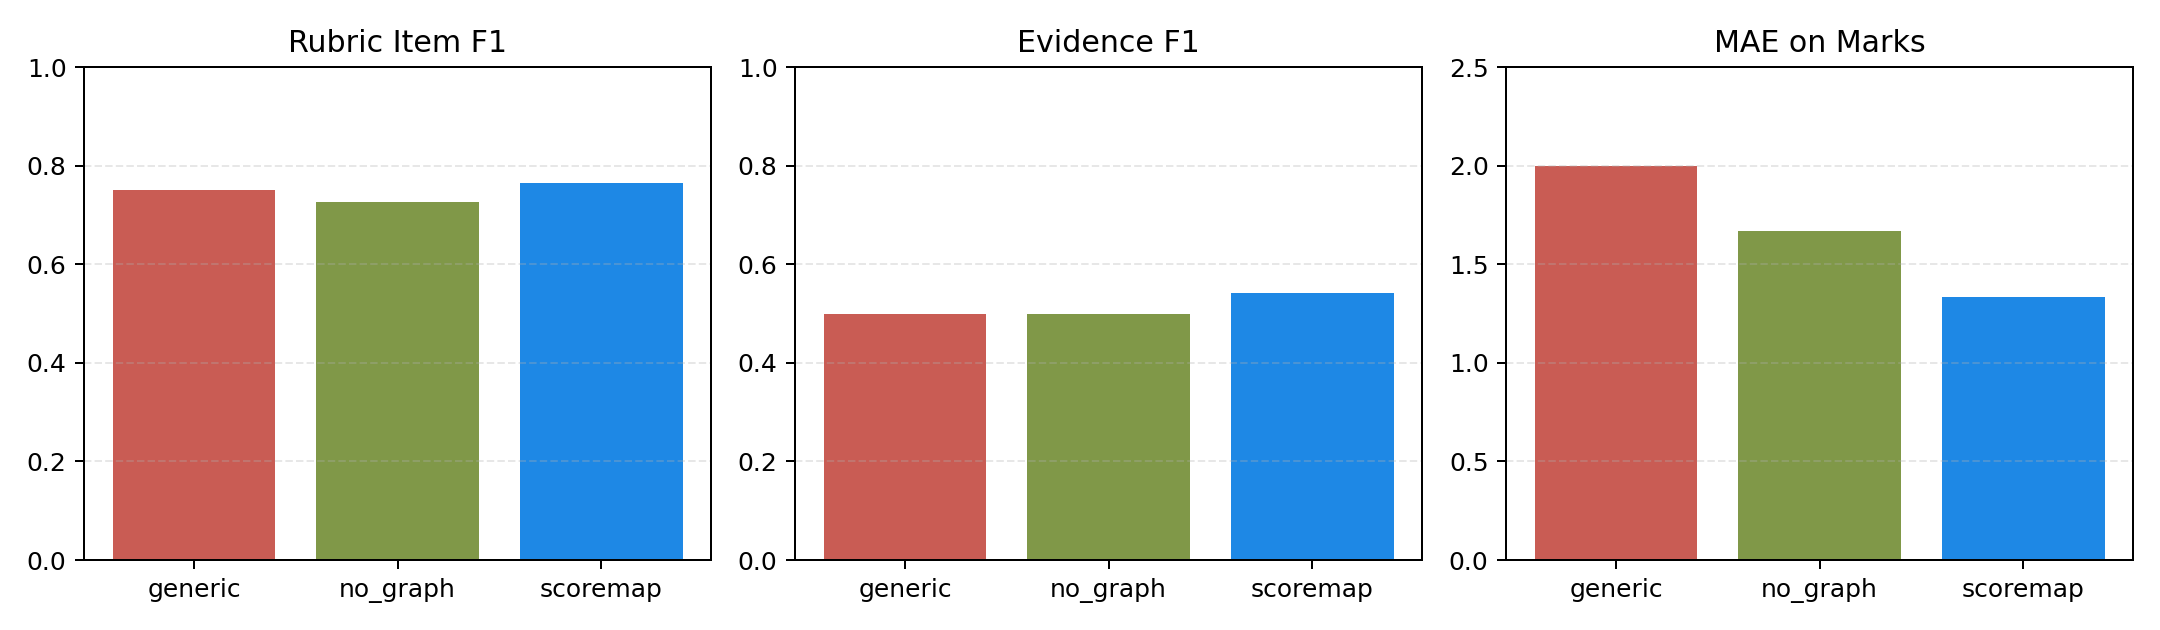
\includegraphics[width=0.9\linewidth]{figures/model_comparison.png}
\caption{Model comparison on the pilot benchmark.}
\label{fig:comparison}
\end{figure}
\section{Failure Cases and Limitations}
Current limitations include unsupported diagram families, terse answers, and reliance on region-level text in the included lightweight prototype.
\bibliographystyle{plain}
\bibliography{references}
\end{document}